\chapter{Chiffrement RSA}

\section{Écrire un programme d'exponentiation rapide}

L'exponention rapide est une méthode permettant de calculer rapidement des grandes puissances de nombre. En effet, pour calculer de manière naïve $n^p$ avec $p$ très grand, c'est-à-dire en multipliant $n$ par lui-même $p$ fois, est très peu efficace.

Explication de l'algorithme :\\

Sur la figure \ref{fig:perf_exp_rapide}, on peut voir la différence de performance entre l'algorithme naïf (avec des multiplications successives) et l'algorithme d'exponentiation
binaire. Pour 10 itérations de $2^{1000000}$, l'algorithme naïf prend 168.49 secondes alors que l'algorithme d'exponentiation binaire prend 0.04 secondes. \\

\begin{figure}[H]
\centering
    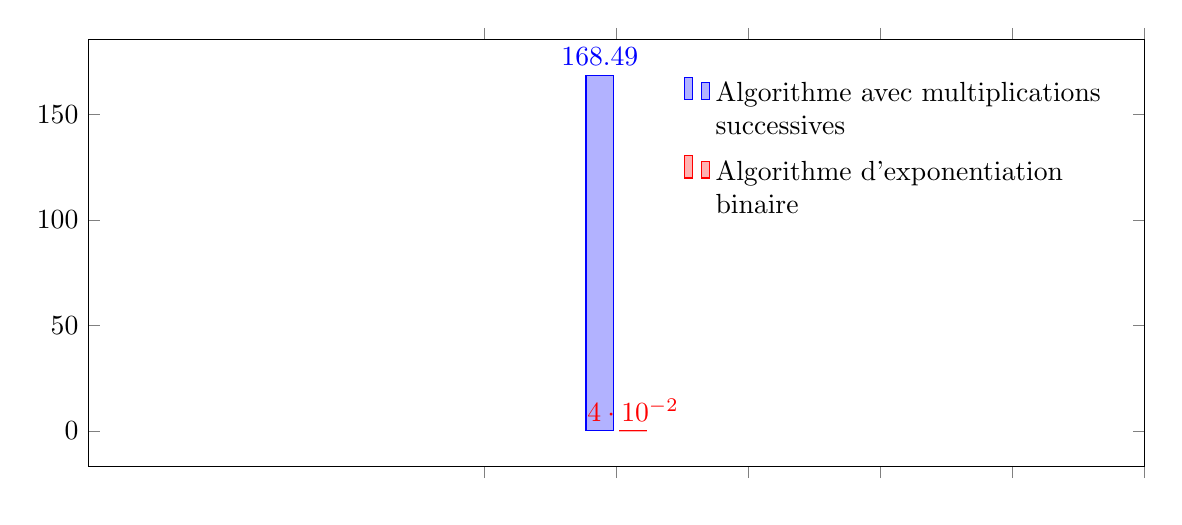
\begin{tikzpicture}
    
        \begin{axis} [
            ybar,
            nodes near coords,
            width=15cm,
            height=7cm,
            xticklabel=\empty,
            legend style={
                draw=none,
                text width=5cm,
                minimum height=1.0cm,
            }
        ]
        \addplot coordinates {
            (1,168.49)
        };
        \addplot coordinates {
            (1,0.04)
        };
        \legend {Algorithme avec multiplications successives, Algorithme d'exponentiation binaire};
        \end{axis}

    \end{tikzpicture}
\caption{Comparaison des performances des 2 algorithmes pour 10 itérations avec $2^{1000000}$} \label{fig:perf_exp_rapide}
\end{figure}


BONUS : autres implémentations : https://stackoverflow.com/questions/9434183/whats-the-fastest-algorithm-to-perform-exponentiation

\section{Écrire un programme de calcul des coefficients de Bézout}



\section{Écrire un programme de chiffrement RSA}